
\newcommand{\dolphinscheduler}{\textit{DolphinScheduler}}
\newcommand{\rocketmq}{\textit{RocketMQ}}
\newcommand{\argouml}{\textit{ArgoUML}}

\section{Experiment 2: ChatGPT suitability evaluation}\label{sec:metric_based_eval}

As the first experiment shows the limitations of ChatGPT while detecting and refactoring data clump, these results center on human feedback which is subject to bias and other uncontrollable influences. 

To further evaluate the usefulness of ChatGPT in the pipeline, a second experiment was conducted.

In this second experiment, tests were conducted to assess the suitability of ChatGPT performing steps of the pipeline. In contrast of the first experiment, this experiment is centered on a limited set of projects and uses more metrics while leaving out human feedback. These experiments center on RQ 2 which deal with suitability of ChatGPT in the refactoring pipeline and RQ 3 which is about the effect of \ac{LLM} parameters. Both of these research questions are answered in this experiment. 

Since the pipeline consists of several steps where the model can be used, the experiment was split into  four sub-experiments (numbered from 2A to 2D) where each sub-experiment is independent from the other. Each experiment deals with a distinct part of RQ 2 and 3. 

The following steps from the pipeline were considered:

\begin{itemize}
    \item Detect data clumps
    \item Filter data clumps
    \item Refactor data clumps
\end{itemize}

Table \ref{tbl:expB} shows the derived research question of each experiment and the identifier of the experiment. 
\begin{table}[ht!]
    \centering
    \begin{tabular}{m{2cm}|m{10cm}| m{2cm}}
      Experiment   & RQ answered & Step in the pipeline  \\\hline
        2A & How well can ChatGPT detect data clumps? & Detect  \\\hline
        2B & How well can ChatGPT detect data clumps that the \textit{DataClumpDoctor} could not detect? & Detect \\\hline
        2C & How well can ChatGPT choose the best data clump for refactoring? & Filter \\\hline
        2D & How well can ChatGPT  refactor data clumps? & Refactor \\\hline
    \end{tabular}
    \caption{Overview about experiments}
    \label{tbl:expB}
\end{table}

Each of these experiments answers a derivation of RQ 2 as well as a derived third RQ. For instance, In experiment 2A, the RQ answered deals with the detection capability of ChatGPT. At the same time, the influence of different \ac{LLM} parameters on the detection capability is tested. 

\subsection{General methodology}

In contrast to the feedback-based experiment, multiple data clumps are selected that will be used in the succeeding steps. These data clumps are not chosen manually as in the first experiment but selected via an algorithm. This algorithm is as follows:
\begin{enumerate}
    \item Select 
\textit{n}
 data clumps based on one criterion, and 
\textit{n}
 data clumps based on another criterion, and so forth.
    \item Determine the total file size of the files affected by this set of data clump.
    \item Save this set of data clumps if its file size is smaller than the current minimum.
    \item if the current minimum has not improved for 1000 iterations, return the minimum and the associated data clumps.
\end{enumerate}

With this local optimum search strategy, a set of data clumps is retrieved that can be used as the basis for the detection, filtering and refactoring step while also minimizing the total file size transmitted to the \ac{LLM}. 

The exact criteria and amount of data clumps used for the data clump selection depend on the concrete experiment. For instance, if the best data clump should be chosen by the model, very large data clumps and data clumps affecting many classes and methods should be transmitted. This creates a stark contrast between the proposed data clumps and forces the model to make a genuine selection for a suitable data clump. In the refactoring step only two random data clumps were considered  because it could be expected that subsequent validation steps would increase the amount of transmitted data even more. Hence, submitting more files would increase the likelihood of context window overflow. This issue does not occur under the detection and filtering step. 

\subsubsection{Selection of projects}

Selecting projects for this experiment was easier because no human feedback was required so that the active maintaining criterion in section \ref{sec:github_projects} is not relevant. However, the other criteria were still relevant. 

As a result, projects were selected that have already been used for experiment regarding code smells or refactoring in the literature. The following list shows the selected projects together with a description:
\begin{description}
    \item[ArgoUML:] Open source UML modeling tool. \cite{argouml}
    \item[RocketMQ:] A cloud-native messaging, eventing, streaming real-time data processing platform. \cite{rocketmq}
    \item[DolphinScheduler:] A distributed and extensible open-source workflow orchestration platform. \cite{dolphinscheduler}
\end{description}


\subsubsection{Parameterization}

In order to answer RQ 3, multiple \ac{LLM} parameters must be considered.  These parameters determine how the model can interpret the instruction and how it should respond. Using different hyper-parameters can show whether special care should be given to these parameters or whether they are irrelevant. The following parameters are considered: 

\begin{description}
	\item [Temperature:] This parameter describes the randomness of the output of the model. The less temperature, the more the output is predictable. However, this reduces the model's potential for creating creative output.
	
	%\item[Instruction type] This parameter describes how the concept of data clump is taught to the model. Three types are tested: In the definition-based approach a formal definition resembling the definition given in section \ref{sec:data_clump_def} is provided. In contrast using the no-definition method, the term \enquote{data clump} is not explained at all so that the model must use its inherent knowledge. A third option is to provide examples of data clumps In Java which requires the model to learn this concept by analyzing similairities in source code.  
	
	\item [Input format:] This parameter is discussed in section \ref{sec:input_format}. The available values for this parameter depends in what steps of the pipeline the model is used. For instance, in the detection step, the data clump type context is not available and cannot be submitted to the model. In the refactoring step, only source code can be submitted as that source code must be changed by the model.
	
	\item [Margin:] This parameter is only relevant if code snippets are transmitted. In other cases, it would have no effect since it only affect the size of the code snippets. Values considered here are 0, 1, 2, 5 and 10, 
	
	
\end{description}

Other parameters that could be considered are the model, which has a great impact on the output, the output format, the specific model, and the concrete instruction given to the model. However varying too many parameters can be a significant obstacle to evaluate the experiments so that only these parameters are used. 

For each parameterization, the experiment was repeated ten times. 



\subsubsection{Metrics}

To evaluate the quality of \ac{LLM} in the pipeline, several metrics are employed that give an hindsight about the potential of such models. These metrics return a numerical value. These metrics are not scaled to a uniform range. The metrics can be further categorized into common metrics and experiment-specific metrics. 


Common metrics are used by each experiment as they are not specific to a specific experiments and can be evaluated by all experiments. These metrics include
\begin{description}
    \item [Price:] The total price in US-Dollars of a query which includes the price for processing the input and the price for the output
    \item [Time:] The time needed from sending the query to the \ac{LLM} server until it responds. 
    \item[ Data-clump-specific:] Attributes of the data clump considered by the model. This includes the size, occurrence, affected files of the respective data clump. 
    \item[Validity of the JSON:] This metrics determines whether the output of the \ac{LLM} is valid \ac{JSON}. Invalid output can occur if the model hallucinates or the output is too large.
\end{description}


On the other hand, experiment-specific metrics do only apply to a specific experiment and would not make sense for all experiments. These metrics are discussed in the subsections for each individual test. 

For brevity reasons, the results of every metric are not discussed in this master's thesis. All data such as figures or raw data is available in the directory \enquote{experiment1} of the digital appendix. 


\subsection{Experiment 2A: Data clump detection}

Detecting data clumps is an essential part to refactor them. Because it happens at a very early state in the pipeline, it is even more important that the data clump detection data is accurate and conforms to the specification. The question here is whether the model can perform this task so that subsequent steps of the pipeline (e.~g. a manual refactoring tool) can rely on the data. If the reliability of the results is too low, it becomes more challenging to develop  handlers that can handle with possibly erroneous data.

Additionally, in contrast to a manual tool, detecting data clumps via  a model might also include a filtering process because the model might not return all data clumps but only a subset of them. This means that further filtering in subsequent steps might not be necessary. 

The format presented in appendix \ref{app:data_clump_format} is used as the output format because subsequent handlers have been adapted on this context. 


\subsubsection{Methodology}

For this experiment, either code snippets or complete files are submitted, and the model is asked to find all data clumps and to report its result in the specified format.
Because transmitting the full project is infeasible, the data clumps are previously detected using the \textit{DataClumpDoctor}. The relevant locations of the most important data clumps are then used as a basis to submit the request to the model. In case of code snippets, this would mean that the code snippets only contain data clumps and no other parts of the source code. As this might induce a bias, all other methods in the respective file having at least three parameters are included too. Also, all fields in a class are submitted if such a class has at least three fields. As a result, the model still has to identify the correct data clump while  the transmitted tokens are minimized.  


The following metrics are used for evaluating this test:

\begin{description}

    \item[Correctness of output format:]
    As already noted, the correctness of the output format representing the data clump is essential. If the model reports in wrong format, the data must be interpreted again which increases the risk of faults complicates integrating the \ac{LLM}. This metric counts the number of deviations from the required output format.

     \item [Surety of the results:] In contrast to the preceding metric, not the exact output format is analyzed but the correctness of the entailed data. For instance, the model might return a wrong line number or method name which would have a significant impact on succeeding steps. This metric is calculated by subtracting the number of wrong information from the number of correct information. 

     \item [Number of data clumps:] This metrics describes how many data clumps are returned by the model. It does not differentiate whether these data clumps are virtually identical or whether they are data clumps at all. 
     

   

    

   
\end{description}



\subsubsection{Results} 

The experiment shows the limitation of the output format even with some simplifications. On average, only three data clumps are returned which is not enough to cover all data clumps in the chosen projects. This is further highlighted by the \ac{JSON} validity metric which is about 80 percent. However, the output format correctness is high with a median of at least 80~\%. 

Considering the effect of the temperature, the number of detected data clumps decreases with higher temperature while  the \ac{JSON} is more often valid. At the same time, the costs and the processing time decrease because fewer token are output. There is an inconclusive effect of the temperature on the surety. The surety decreases with rising temperature for \textit{RocketMQ} and \textit{Dolphinscheduler} while it increases in the case of \textit{ArgoUML}. 

The effect of the input type is also visible. Providing full files instead of code snippets decreases the surety.  Figure \ref{fig:detect_input_surety} compares the surety of both input formats via a box plot. The left box plot visualizes the surety if code snippets are provided. The surety has a median of 2.5. Additionally, the upper whisker has a value of 7.5, while the lower whisker has a value of -4.25. There is only one outlier.

On the other hand providing full source files results in a smaller median of 1.0 as the right box plot shows. This box plot is more compact showing less variance within its interquartile range.  Additionally, there are more outliers which even reaches a surety of -15.  Since the surety is defined as the number of information that is correct minus the number of incorrect information, it can be seen that providing full source files is less reliable and results in more mistakes by the model. 



\begin{figure}[ht!]
    \centering
    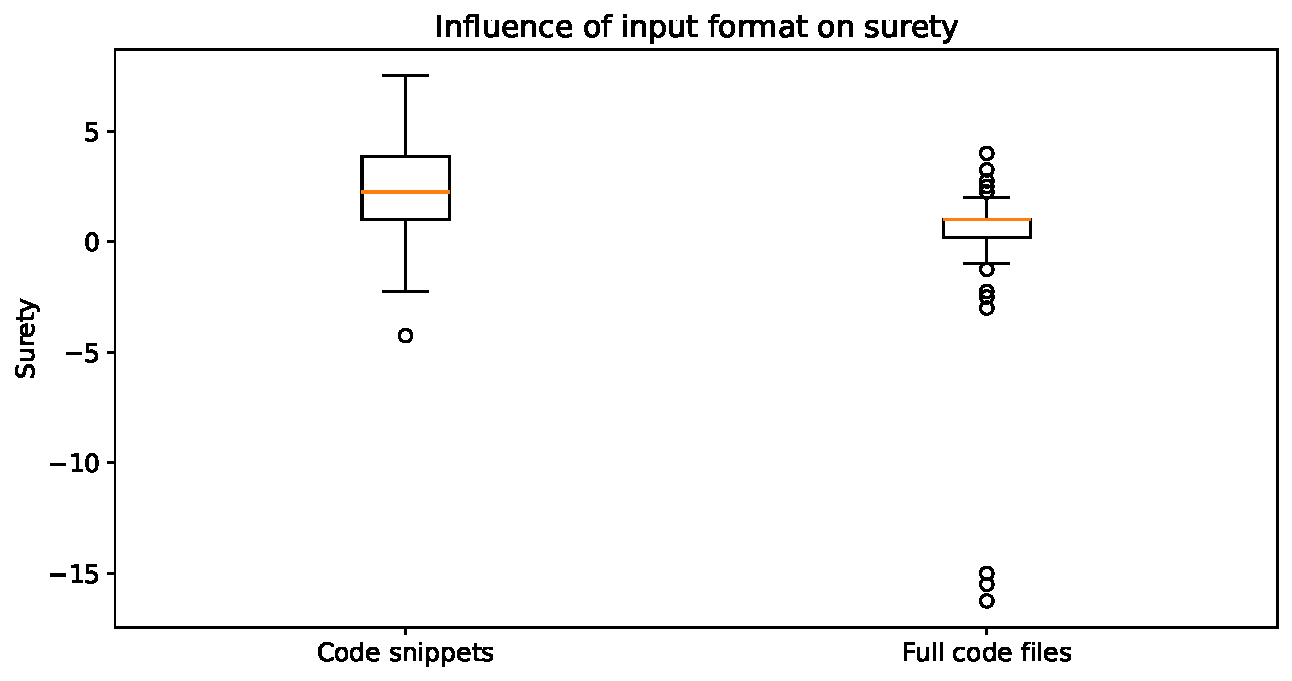
\includegraphics[width=\columnwidth]{figures/chapter5/detect_input_format_surety.pdf}
    \caption{Boxplot: Influence of input format on Surety}
    \label{fig:detect_input_surety}
\end{figure}

Analyzing the time needed to fulfill a request, it can be seen that some waiting time should be taken into account. The boxplot in figure \ref{fig:temperature_time} shows how the temperature of the model influences the processing time. The median time  decreases with increasing temperature. For instance, the median time for a temperature of 0.1 is nearly 100 seconds while it is nearly 50 seconds in the case a temperature of 0.9. Also, the upper whisker decreases from 250 to 150 while the lower whisker also decreases slightly. The existence of a multitude of outliers on the upper bound shows that the server response time can vary significantly. 

\begin{figure}
    \centering
    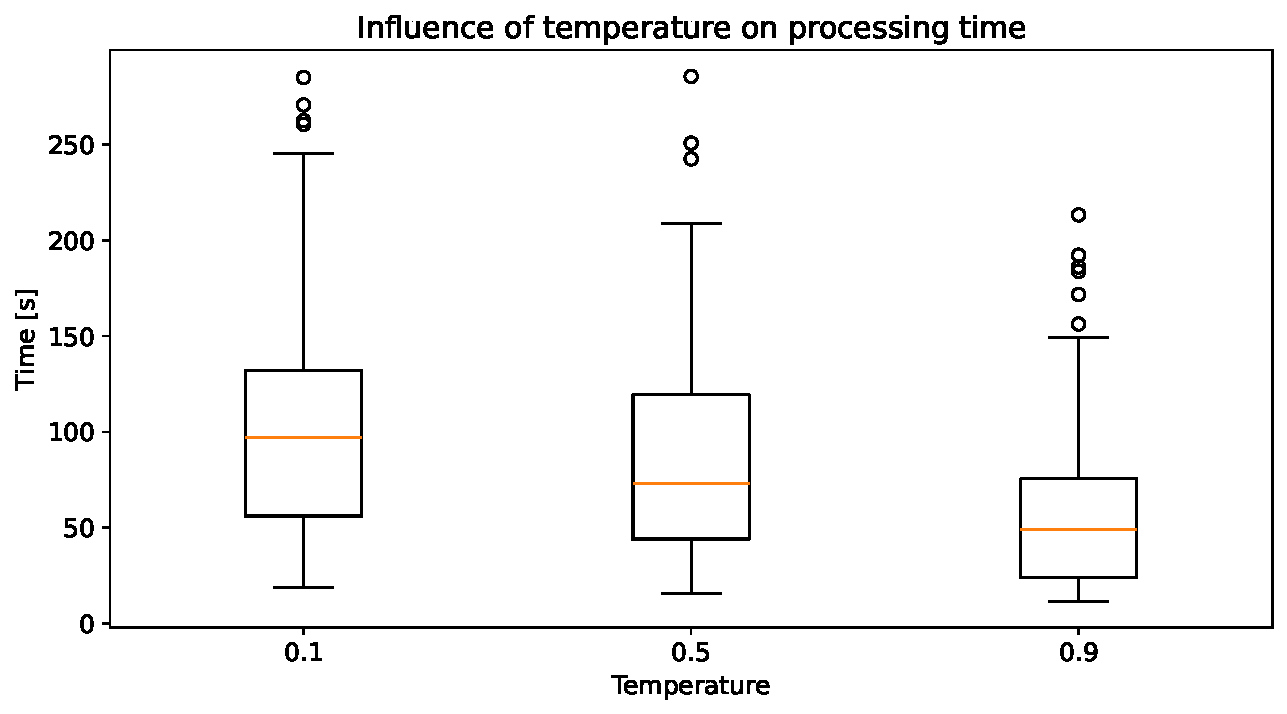
\includegraphics[width=\columnwidth]{figures/chapter5/detect_temperature_time.pdf}
    \caption{Boxplot: Influence of temperature on time}
    \label{fig:temperature_time}
\end{figure}

\subsubsection{Threats to validity}

In the detection experiment, the returned data clump type context is linked to the real data clump type context to determine which data clumps are detected. The metric finds the real data clump that shares the most similarities with the returned data clump. However, this could be a completely wrong data clump. For instance, if the model returns a correct class name containing a data clump but otherwise is wrong, it is still considered for the data clump type, size, and occurrence metric. The accuracy of the information is only considered in the surety metric.

Additionally for the output accuracy metric, the relevance of each parameter in data clump type context is disregarded. For instance, the data clump type context contains information about the line number of each data clump. Even if this information is missing, it can be replaced by considering the other information (variable names, method name, class name). 



\subsection{Experiment 2B: Data clump detection with modifications}

This experiment is a derivation from the preceding one. Similarly to the detection experiment, the goal is to detect data clumps in a software project.

However, now the source code is modified to test whether the model can detect data clumps that the \textit{DataClumpDoctor} would miss due to difference in the names or data types of the clump items. Three types of modification should be distinguished:

\begin{description}
    \item[Synonym:] A synonym of variable name is used. For instance, the words \textit{change} and \textit{modification} have a very similar  meaning. 

    \item[Typographical error:] A spelling error resulting in a slightly modified name. This could be caused by a developer not knowing the exact spelling of a word. However, it could also happen by accident if the developer mistypes while writing the source code.

    \item [Type mismatch:] Two variables that share the exact names but have a similar type .
\end{description}

In each of these cases, it can be argued that a data clump can still exist even with these modifications. For synonyms and type mismatches however, allowing such changes might increase the chance of false positives. 

\subsubsection{Methodology}

For this experiment, data clumps with exactly three items were randomly sampled. For each data clump, one modification was introduced (e.~g. replacing the name of a variables by a synonym), if such change was reasonable.

It is important to only consider data clumps with exactly three items because  a modification of one item would invalidate the data clump for a traditional tool like the \textit{DataClumpDoctor}. If larger data clumps were to be submitted, the model could return only a subset of the data clump items and ignore the item with the modifications. 

To find synonyms for a given word, the WordNet \cite{10.7551/mitpress/7287.001.0001} library was used. This library can find similar words to a given word.

To find typographical errors, the Birbeck database \cite{birbeck} was used which contains spelling mistakes in the English language. From this database, a spelling mistakes was chosen that could reasonably happen to a developer (e.~g. writing a letter twice, omitting a letter etc.). 

Type modifications were only performed on numerical types such as \textit{int}. For instance,  the type \textit{long} might be replaced by \textit{int}. 

The same metrics as in the detection experiment are used. Additionally, it is counted how often the model detects a data clump with a modification. 





\subsubsection{Results}

In summary, ChatGPT was able to detect data clumps with synonyms and typos while facing enormous challenges identifying data clumps with different types. However, the capability of ChatGPT ignoring such modifications varies strongly between projects. 

\begin{figure}[ht!]
    \centering
    \begin{subfigure}[t]{0.44\columnwidth}
        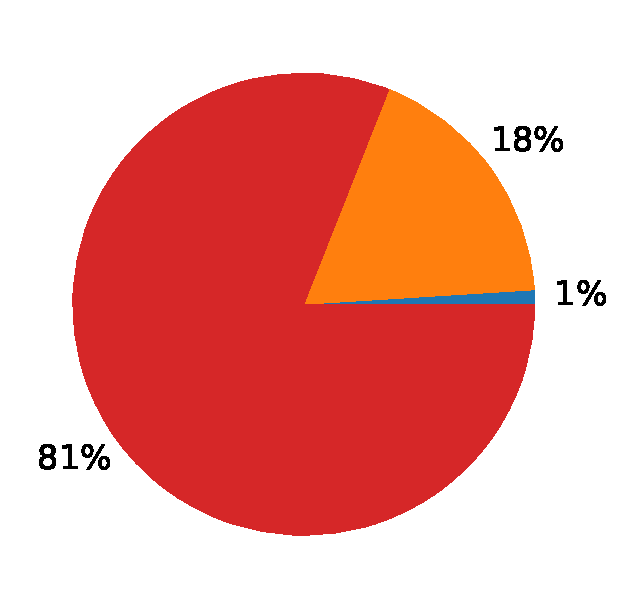
\includegraphics[width=0.8\columnwidth]{figures/chapter5/detectSyn_mod_type_argouml.pdf}
        \caption{ArgoUML}
        \label{fig:detect_syn_mod_type_argouml}
    \end{subfigure}
            \begin{subfigure}[t]{0.44\columnwidth}
        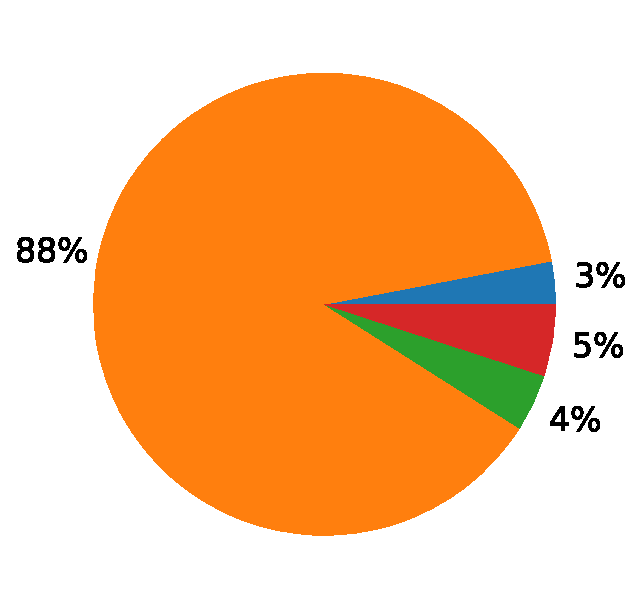
\includegraphics[width=0.8\columnwidth]{figures/chapter5/detectSyn_mod_type_rocketmq.pdf}
        \caption{RocketMQ}
       \label{fig:detect_syn_mod_type_rocketmq}
    \end{subfigure}
        \begin{subfigure}[t]{0.5\columnwidth}
        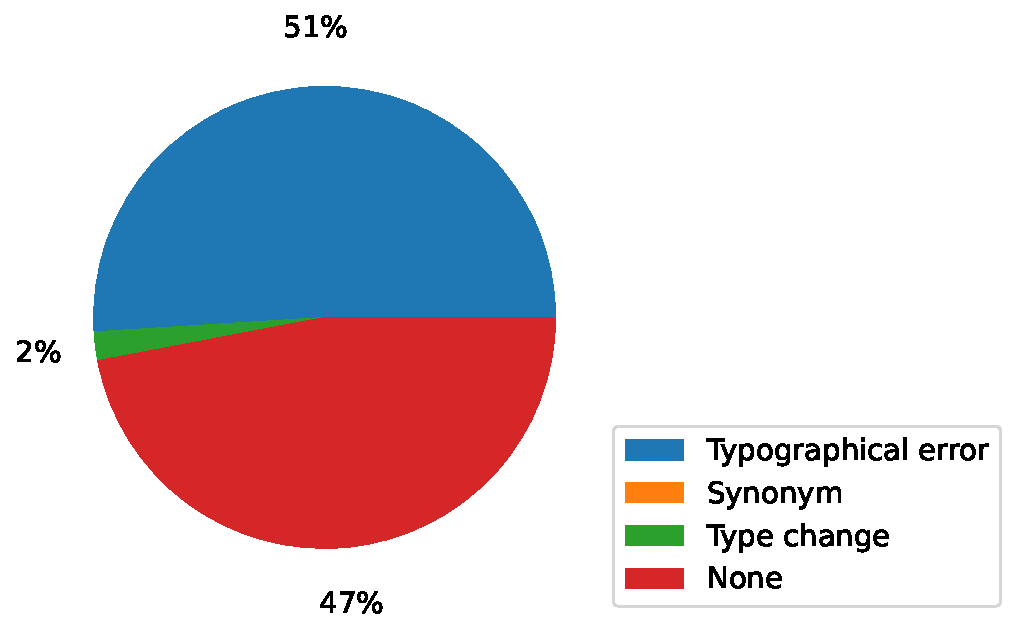
\includegraphics[width=1.2\columnwidth]{figures/chapter5/detectSyn_mod_type_dolphin.pdf}
        \caption{DolphinScheduler}
        \label{fig:detect_syn_mod_type_dolphinscheduler}
    \end{subfigure}

    \caption{Types of detected data clumps with modifications by project}
    
    \label{fig:detect_syn_mod_type}
\end{figure}


 The pie diagrams  \ref{fig:detect_syn_mod_type_argouml}, \ref{fig:detect_syn_mod_type_rocketmq}, and \ref{fig:detect_syn_mod_type_dolphinscheduler} depict the percentages of data clump detected by modification type. In the case of \textit{ArgoUML} and \textit{Dolphinscheduler}, 81~\% of the  data clumps detected were not modified. 18~\% of the detected data clumps have a synonym as a modification while the remaining 1~\% of the case belong the category data clumps with typos. No data clumps were detected that have a modified data type. 

 A stark contrast exists for \textit{RocketMQ}. 88~\% of the detected data clumps were modified by using a synonym. In 3~\% of the cases, the data clumps have a typo. A data type was modified in 4~\% of the identified data clumps. In the remaining 5~\%, the data clumps had no modifications. 

For \dolphinscheduler, the ratio of data clump with typos is 51~\% while in 47~\% of the identified data clumps no modifications were applied. In the remaining 2~\% of the cases, a data type was modified. No data clumps with synonyms were detected. 



The input format also has some influence on the category of data clumps detected. Figures \ref{fig:detectSyn_full_files} and \ref{fig:detectSyn_snippets} show the impact of the input format as a pie chart. 

 26~\% of the detected data clumps have a synonym as a modification if full code files are submitted. This value increases to 39~\% if code snippets are provided. On the hand, the percentage of detected data clumps with typos decreases from 21~\% to 17~\%. Also, the number of detected data clumps with data type modifications decreases from 4~\% to 1~\%. Consequently, 49~\% of the detected data clumps have no modifications if complete files are submitted while this value is 43~\% in the case of code snippets.  

\begin{figure}[ht!]
    \centering
    \begin{subfigure}[t]{0.5\columnwidth}
        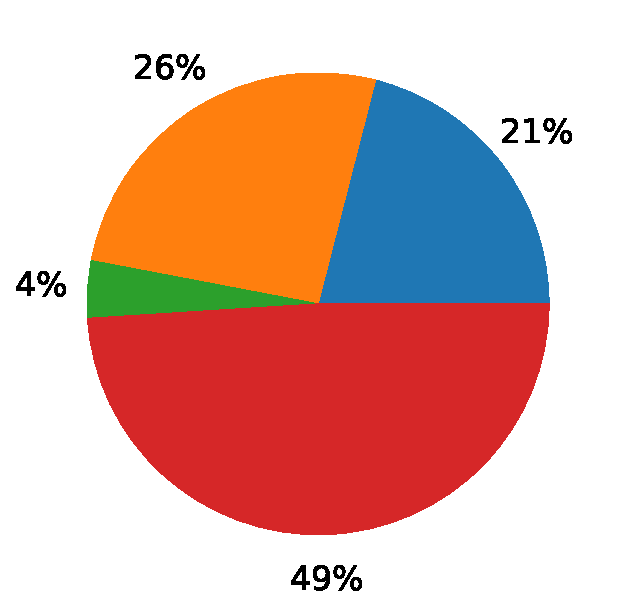
\includegraphics[width=0.8\columnwidth]{figures/chapter5/detectSyn_input_fullFile.pdf}
        \caption{Full code files}
        \label{fig:detectSyn_full_files}
    \end{subfigure}
            \begin{subfigure}[t]{0.5\columnwidth}
        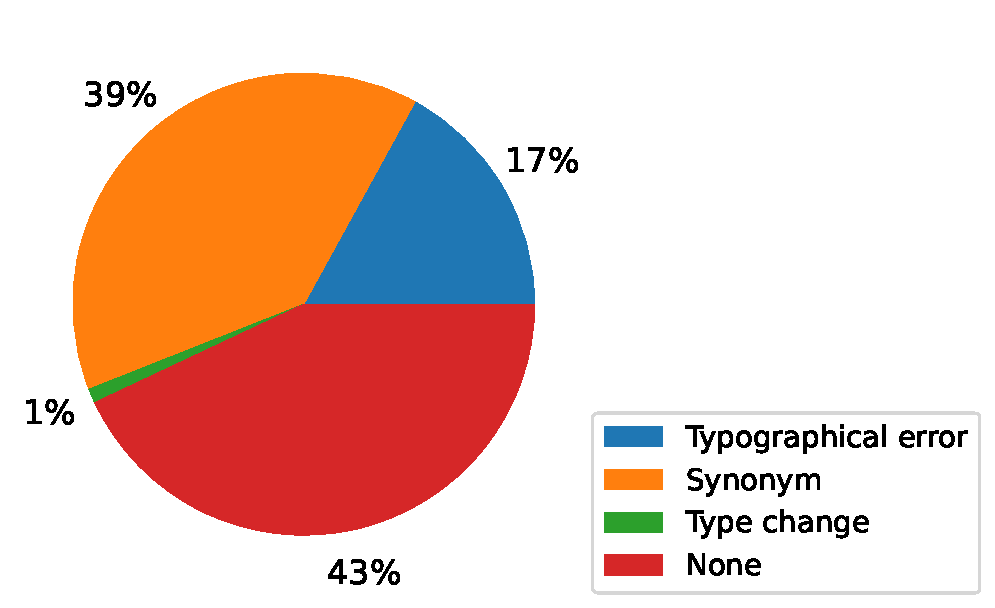
\includegraphics[width=1.3\columnwidth]{figures/chapter5/detectSyn_input_snippet.pdf}
        \caption{Code snippets}
       \label{fig:detectSyn_snippets}
    \end{subfigure}
       

    \caption{Types of detected data clumps with modifications by input format}
    
    \label{fig:detect_syn_input_type}
\end{figure}

\subsubsection{Threats to validity}
In general, the Threats to validity from the detection experiment apply here too. 

Additionally, the concrete modification applied to a data clump item can strongly affect the result. For instance, the Birbeck dataset contains mostly spelling mistakes made by children or illiterate adults so that developers could possibly make other mistakes which would be easier to spot for a model. 

Also the WordNet database is not specialized on technical terms but is more general. This means that the synonyms chosen here might not be synonyms used by a developer.

\subsection{Experiment 2C: Data clump filtering by model}

The filtering experiment is somewhat similar to the detection experiment. However, here the model is told to return one data clump that is most relevant. Additionally, it does not need to use the data clump type context as the output format because this information already exists. 

As outlined in section \ref{sec:data_clump_filtering}, there are multiple approaches for filtering data clumps, which can already be implemented manually. 
The question here is whether the \ac{LLM} uses novel filtering approaches or simply relies on the metric discussed in section \ref{sec:data_clump_filtering}. In the latter case, it is more useful to use the manual algorithm because they are reliable and do not incur the costs associated with Large Language Models. 

\subsubsection{Methodology}

This experiment is conducted similarly to the detection test. However, at this time, the data clump type context as outlined in appendix \ref{app:data_clump_format} is included as a possible input format. Additionally, if code snippets are provided, they always contain data clumps as opposed to possible data clumps as outlined in the detection experiment. 
The output format is discussed in section \ref{sec:output_format_filtering}
The following metrics are used to evaluate this experiment:
\begin{description}
    

    \item [Surety:] This metric is identical to the surety metric in the detection experiment. 
    \item [Reason:] A reason given by the model that explains why the model chose a particular data clump. 
    \item [Position on ground truth:] The minimal index of the data clump with respect to the occurrence, size, and affected files metrics.
\end{description}


\subsubsection{Results}

Figures \ref{fig:filter_reason_argouml}, \ref{fig:filter_reason_rocketmq}, and \ref{fig:filter_reason_dolphinscheduler} visualize the distribution of the reason provided by the model as a pie diagram.

For \argouml, in 42~\% of the cases, the model named the number of affected files as the reason to return a specific data clump. In 15~\% of the cases, the size of the data clump was the most important factor. The occurrence mattered in 13~\% of the cases. In the remaining 30~\% of the cases, the \ac{LLM} chose the data clump because of the domain of the variables. 

Considering the project \rocketmq, it can be seen that the percentage of the reason \enquote{Affected files} is also relatively large with 33~\%. Additionally, the occurrence was mentioned in 38~\% of the cases. In 19~\% of the filtering proposals, the size of the data clump was named as the reason for refactoring. Lastly, the domain of the data clump variables was specified as the model's choice in 10~\% of the cases.

In the case of \dolphinscheduler, the importance of the domain is greater since 36~\% of the suggestions named this reason. Additionally, the affected files played a less role as the percentage is 14~\%. The same applies to the reason \enquote{size} which is 4~\%. On the other hand, the occurrence of the data clump remained an important reason for the model as it was named in 46~\% of the cases. 
\begin{figure}[ht!]
    \centering
    \begin{subfigure}[t]{0.48\columnwidth}
        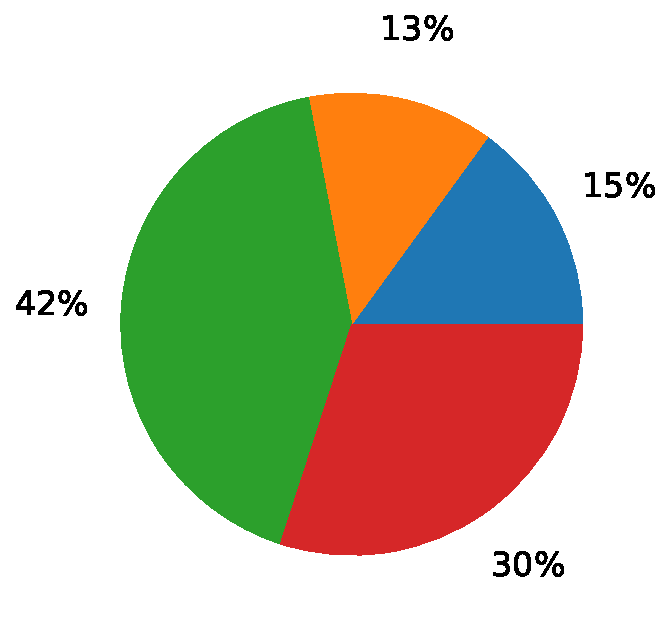
\includegraphics[width=1\columnwidth]{figures/chapter5/filter_reason_argouml.pdf}
        \caption{ArgoUML}
        \label{fig:filter_reason_argouml}
    \end{subfigure}
            \begin{subfigure}[t]{0.48\columnwidth}
        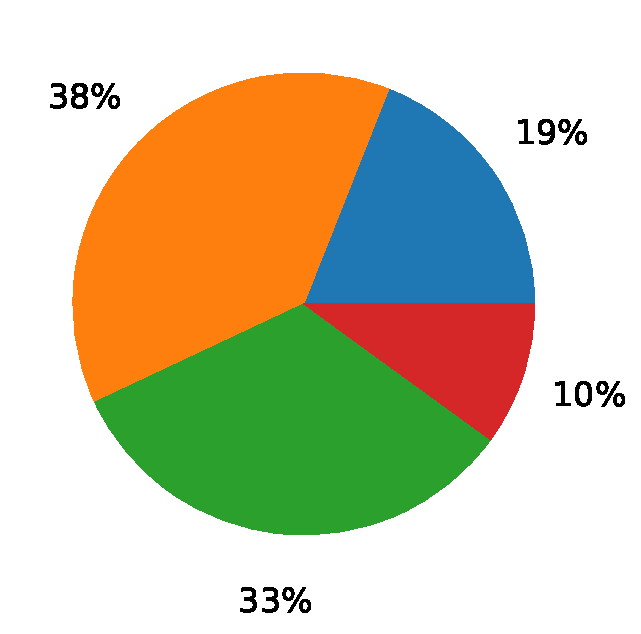
\includegraphics[width=1\columnwidth]{figures/chapter5/filter_reason_type_rocketmq.pdf}
        \caption{RocketMQ}
       \label{fig:filter_reason_rocketmq}
    \end{subfigure}
        \begin{subfigure}[t]{0.6\columnwidth}
        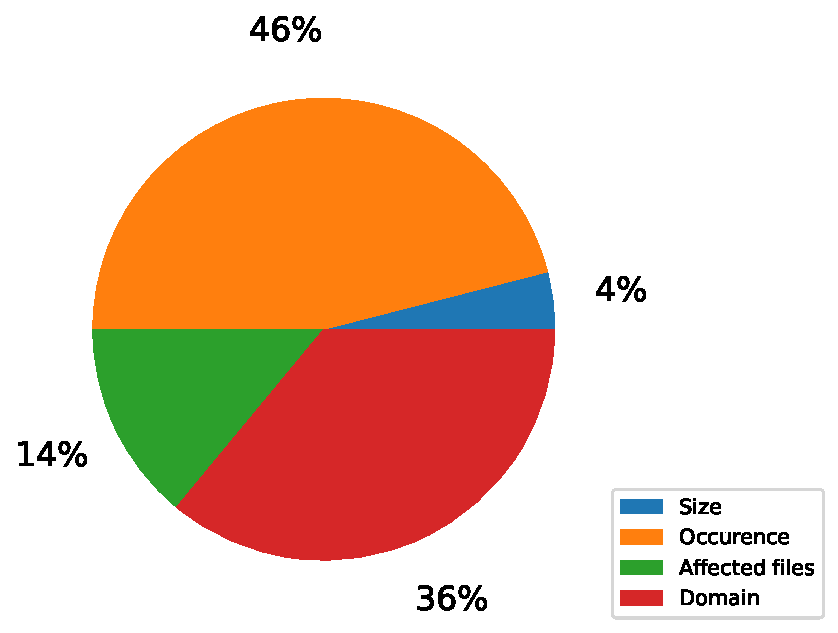
\includegraphics[width=1.3\columnwidth]{figures/chapter5/filter_reason_type_dolphin.pdf}
        \caption{DolphinScheduler}
        \label{fig:filter_reason_dolphinscheduler}
    \end{subfigure}

    \caption{Distributions of reasons for selecting a data clump provided by the model }
    
    \label{fig:filter_reason}
\end{figure}

The position on the ground truth varied per project. The box plot in figure \ref{fig:filter_project_posgroundtruth} visualizes the distribution.  

For \argouml, the median is zero and no whiskers  are visible. However, a multitude of outliers up to 12 are present. This means that in most cases, the model chose the same data clump as a traditional metric. 

On the other hand, \rocketmq shows that the model could choose other data clumps. Here, the lower whisker is 0 while the upper whisker is  3, The median is 2 meaning that the model more often returned a data clump that a traditional algorithm would not suggest.

For \dolphinscheduler, the median is also 2 though in this case no whiskers are visible. This indicates that here also the model would return data clumps more difficult to detect via a classical algorithm. 
\begin{figure}
    \centering
    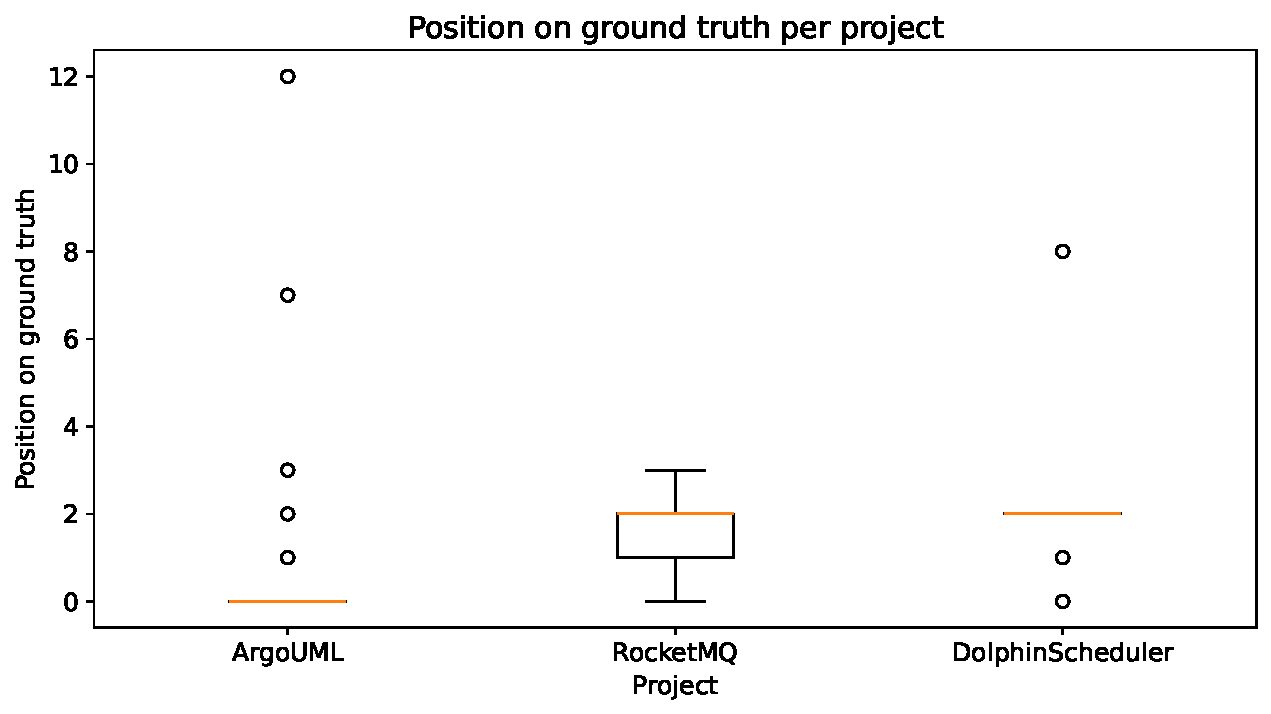
\includegraphics[width=\columnwidth]{figures/chapter5/filter_project_position_groundtruth.pdf}
    \caption{Position on ground per project}
    \label{fig:filter_project_posgroundtruth}
\end{figure}


\subsubsection{Threats to validity}

One threat of validity is   that only one data clumps is returned although it might make sense to return more (e.~g. three). Additionally, as a result of the similarity to the detection experiment, the flaws of the former can be flaws of the latter experiment. 

Moreover, the reason returned by the model should be taken with a grain of salt. The model might claim that is chooses a specific data clump because of its domain but in truth it might have applied other criteria. Hence,  is impossible to verify the reason


\subsection{Experiment 2D: Data clump refactoring}

Evaluating how an \ac{LLM} performs data clump refactoring is another method to assess the suitability of the models for use in the pipeline. Here, especially the creativity is important. If a model merely refactors similarly to a manual tool (e.~g. IntelliJ), it has less use.

If, however, the \ac{LLM} extracts more functionality by creating new methods or solves the data clump in other ways, the advantages of the model become more obvious.



\subsubsection{Methodology}

In contrast, to the detection and filtering experiment, this experiment included actual modification to the source code. 

The model is instructed to find and refactor all data clumps. 
The model outputs by providing diff instruction as discussed in section \ref{sec:output_processing} and the modifications are applied.  The modified program is tested with the respective build system (Gradle or Maven). If the build fails, the model is provided with error messages and the content of the affected lines, and the model is instructed to fix these issues. If after five attempts, the project still does not compiles, no further attempts are made. 

The following metrics are used for evaluating this test:

\begin{description}
    \item [Compilation attempts:] The number of attempts remaining. For instance, if the model takes four iterations to fix all compilation issues, one iteration is remaining. 
    \item[Final program validity:] Whether a refactored program is compilable at the end. 
   \item [Reference error ratio:] This metric shows the ratio of reference errors over all compiler errors. Reference errors are errors about unknown methods, variables etc.  A reference error can be described as  a \enquote{good} error because it could be fixed more easily. On the other hand, a syntactical error like missing parentheses or non-closed comments are more difficult to handle. 
    \item [Rich class:] Whether the extracted class are more than mere data classes
   
    \item [Removed data clumps:] This metric assesses how many data clumps were removed during the refactoring process

    \item [Removed variables:] In contrast to the removed data clump metric, this metric counts the total number of fields and parameters removed during the refactoring process even if these removals do not lead to less data clumps, 
\end{description}



\subsubsection{Results}

In general, ChatGPT is unable to fully perform the refactoring so that the resulting program does compile and work. However it is able to remove many variables and decrease the code size. Many refactorings however are incomplete so that the data clump still remains partly. 

In about 40 percent of the instances, ChatGPT fails to provide concrete diff instructions which means that the source code cannot be changed given the information provided by the model. This indicates that while the diff instructions are helpful to ease refactoring, the model is not trained enough to fully use their potential. 

Additionally, the extracted class are seldom rich (10 percent) which indicates that generating helpful classes is possible but still limited. 
\begin{figure}
    \centering
    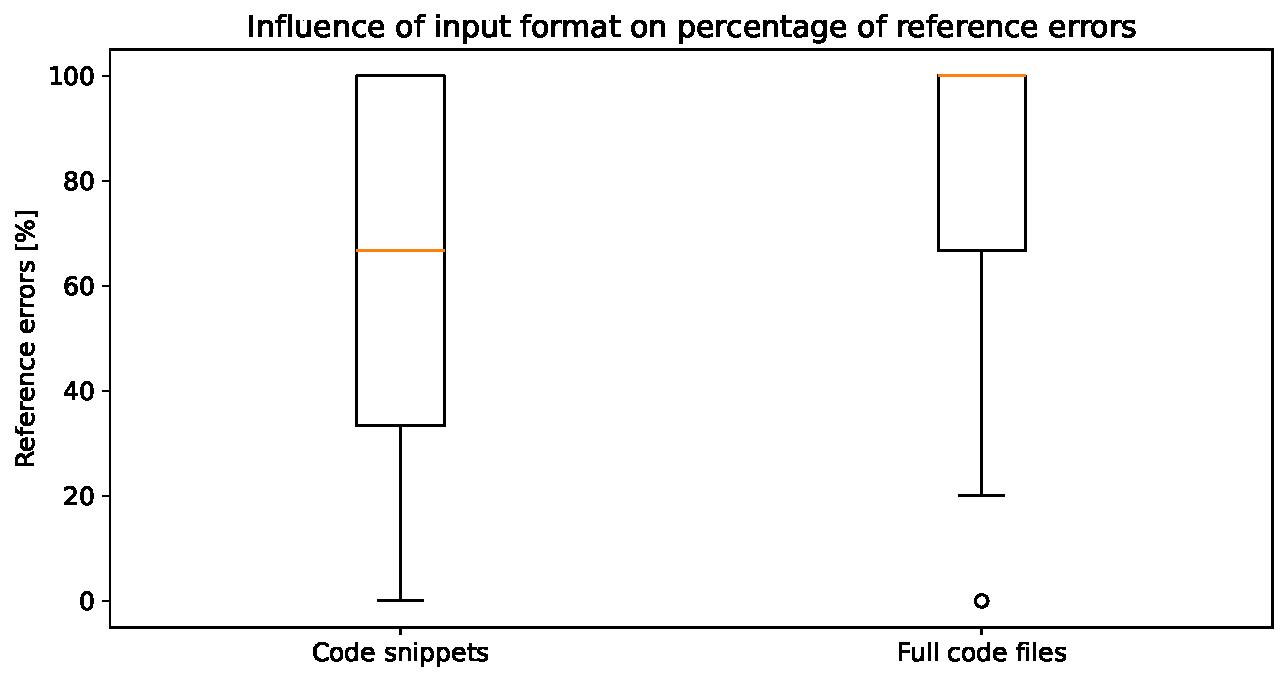
\includegraphics[width=\columnwidth]{figures/chapter5/refactor_input_referenceerrors.pdf}
    \caption{Proportion of reference errors on all errors by input format}
    \label{fig:refactor_input_referenceerrors}
\end{figure}




Additionally, the effect of the input type is visible. Providing full code files decreases the number of valid diff instructions and leads to less removed variables.  Additionally, as figure \ref{fig:refactor_input_referenceerrors} depicts, the complete source code approach leads to less syntactical errors but more errors related to non-updated references (e.~g. method calls).  The left box plot shows a median of about 65~\% and a lower whisker of 0~\% while an upper whisker is not visible. If code snippets are provided, the median increases to 100~\% indicating that syntactical errors are less common. However, the lower whisker is 20~\% which means that such errors can still occur. The outlier at 0~\% further shows that even providing full code files did not prevent major syntactical errors. 


This shows that the snippet approach is not well-handled by the model as it more often introduces syntax errors. 



As for the margin parameters, there is a strong contrast between a margin of 0 and larger margins. For instance, a margin of 0 leads to a high number of non-interpretable diff instructions. Here also, many results are inconclusive and vary between projects. 

Higher margins also led to a decrease in the number of removed data clumps as the box plot in figure \ref{fig:refactor_margin_removedDataClumps} shows. 
For a margin of 0, there is a greater variance. The median is 1 while the upper whisker is nearly 6. The lower whisker is 0. A margin of 1 decreases the median number of removed data clumps and also the value of the upper whisker to about 3. A similar decrease happens if the margin is increased to 2. If the margin is 5 or 10, median becomes 0 while the upper whisker is close to 1. For all margins larger than 0 a significant amount of outliers are present indicating that while data clumps were removed seldom, there were instances where the removal was successful. 
\begin{figure}
    \centering
    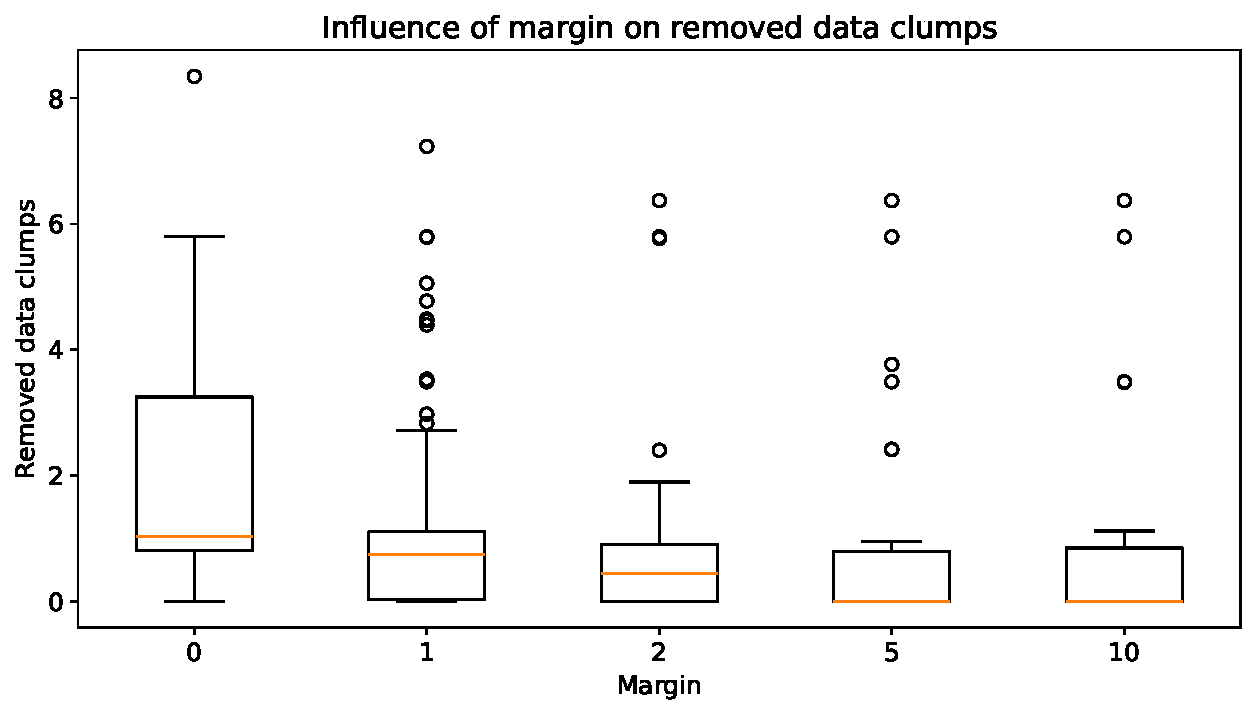
\includegraphics[width=\columnwidth]{figures/chapter5/refactor_margin_removed_data_clumps.pdf}
    \caption{Box plot: Influence of margin on removed data clumps}
    \label{fig:refactor_margin_removedDataClumps}
\end{figure}

\subsubsection{Threats to validity}

For the refactoring experiments, several limitation should be considered. Noteworthy, the number of data clumps transmitted is severely limited as the model should also correct errors which requires retransmitting files multiple times. In many cases, this repeated transmission can exceed the context window so that the number of data clumps (and hence in most cases the number of transmitted files)  needs to be reduced. 

Additionally, in the validation phase, the instruction to fix errors is constant, namely \enquote{Fix all errors in the respective files}. In contrast to a human in the loop who might be able to help the model to solve the compiler errors, the model can only rely on the compiler errors and the content of the files affected by these compiler errors. This can be problematic if the model returns a specific correction output but this output cannot be parsed correctly (e.~g. wrong line numbers). In that case, no compiler errors are fixed and the model might be tempted to use the same output again until the five attempts are exhausted. This problem could only be prevented if concrete feedback is given which is outside of the scope of this master's thesis. 

\subsection{Discussion}



The results from all four experiments show that ChatGPT has potential to be used in the pipeline but many challenges still exists.

As outlined in experiment 2A, The model is capable of detecting some data clumps but due to output size limitation, the number of data clumps is limited. However, the limited number of data clumps might also be a sign of filtering so that non-important data clumps are ignored.

Experiment 2B shows that the model can also detect data clumps that a tool like the \textit{DataClumpDoctor} would not be able to detect. This is useful as a single typo can invalidate a data clump relationship so that a traditional tool would not be able to detect this data clump. This also applies to synonym although one must be cautious as the risk of false positive is higher.

The filtering experiment 2C illustrates that ChatGPT can also find a suitable data clump for refactoring given they have been already detected. This data clump is not always the one proposed by a traditional metric so that other reasons than size or occurrence are used to make a decision on what data clump to refactor. However, as the first experiment shows, the data clump proposed might not be a data clump that a developer wants to refactor. As a result, further investigations about the reasons developer would like to remove data clumps for are warranted.

As for the last experiment 2D,  challenges are clearly visible. While data clumps can be removed by the model, the programs refactored are mostly non-compilable. Additionally, the model is unable to fix those errors which means a human-in-the-loop must intervene. Therefore, automatic data clump refactoring via \acp{LLM} is only imaginable if the model only performs tasks that do not change the source code. A traditional tool like an IntelliJ plugin can then perform the refactoring as it is reliable. 


As to RQ 3, the effect of the parameters can have a significant influence on the quality of the results.  For instance, the code snippet approach is suitable for detecting data clumps while increasing the potential of hard-to-fix errors if it is used for refactoring.
However, other parameters like the margin or temperature do not have a consistent effect on the performance of the model. Hence, practitioners should generate multiple proposals using multiple parameters and  select a suitable one (manually or automatically). This underscores that \acp{LLM} do not always give the best response at first, and comparing multiple solution to a problem (e.~g. multiple data clump refactoring proposals) is one key to improve the integration of \acp{LLM}. 

Further experiments needs to be conducted that analyze the stark difference of parameter's impact on the quality of the results. The observations discussed in  \cite{hallCodeSmellsHave2014} shows a similar discrepancy with regard to data clumps per projects although there it is about the induction of faults.

In summary, it is evident that ChatGPT has some strengths if used in the pipeline which can only hardly be replaced by traditional tools.   For instance, it does not always return the same data clump (e.~g. largest) but uses other metrics in contrast to an approach via classical filters. However, there are many challenges that prevents an fully autonomous refactoring via ChatGPT. 





